%!TEX TS-program = xelatex
%!TEX encoding = UTF-8 Unicode

\documentclass[12pt]{article}       % use "amsart" instead of "article" for AMSLaTeX format
\usepackage{geometry}                       % See geometry.pdf to learn the layout options. There are lots.
\geometry{letterpaper}                          % ... or a4paper or a5paper or ... 
%\geometry{landscape}                       % Activate for for rotated page geometry
%\usepackage[parfill]{parskip} 
%\usepackage{indentfirst}               % Activate to begin paragraphs with an empty line rather than an indent
\usepackage{graphicx}               % Use pdf, png, jpg, or eps§ with pdflatex; use eps in DVI mode
\usepackage{wrapfig}
\usepackage{amsmath}                            % TeX will automatically convert eps --> pdf in pdflatex
\usepackage{amssymb}
\usepackage{amsthm}
\usepackage{cite}
\newtheorem{theorem}{THEOREM}[section]
\newtheorem{lemma}{Lemma}[section]
\usepackage{multirow}
%\usepackage{fontspec}
%\usepackage{xunicode}
%\usepackage{xeCJK}
%\usepackage{fourier}


%\setCJKmainfont[BoldFont={STHeiti},ItalicFont=STKaiti]{STSongti-SC-Light}
%\setCJKsansfont{STHeiti}
%\setCJKmonofont{STFangsong}
%
%\setCJKfamilyfont{zhsong}{STSong}
%\setCJKfamilyfont{zhhei}{STHeiti}
%\setCJKfamilyfont{zhkai}{STKaiti}
%\setCJKfamilyfont{zhfs}{STFangsong}
%\setCJKfamilyfont{zhli}{LiSu}
%\setCJKfamilyfont{zhyou}{YouYuan}
%
%\newcommand*{\songti}{\CJKfamily{zhsong}} % 宋体
%\newcommand*{\heiti}{\CJKfamily{zhhei}}   % 黑体
%\newcommand*{\kaishu}{\CJKfamily{zhkai}}  % 楷书
%\newcommand*{\fangsong}{\CJKfamily{zhfs}} % 仿宋
%\newcommand*{\lishu}{\CJKfamily{zhli}}    % 隶书
%\newcommand*{\youyuan}{\CJKfamily{zhyou}} % 幼圆

\title{Note on transmission and reflection coefficients.}
\author{}
\date{}                         % Activate to display a given date or no date

\begin{document}
\maketitle
\section{Problem setup}

As shown in Figure 1, consider the piecewise linear potential function $V(x)$:
\begin{align}
    &V(x) = s_j(x - x_j) + V_j, \nonumber \\
    &s_j = (V_{j+1/2} - V_{j-1/2})/\Delta x, \\
    &V_j = (V_{j+1/2} + V_{j-1/2})/2, \nonumber
\end{align}
where $j = 0, 1, 2, \cdots, N$ for $x_{j-1/2} < x < x_{j+1/2}$. test

\begin{figure}[htbp]
    \centering
    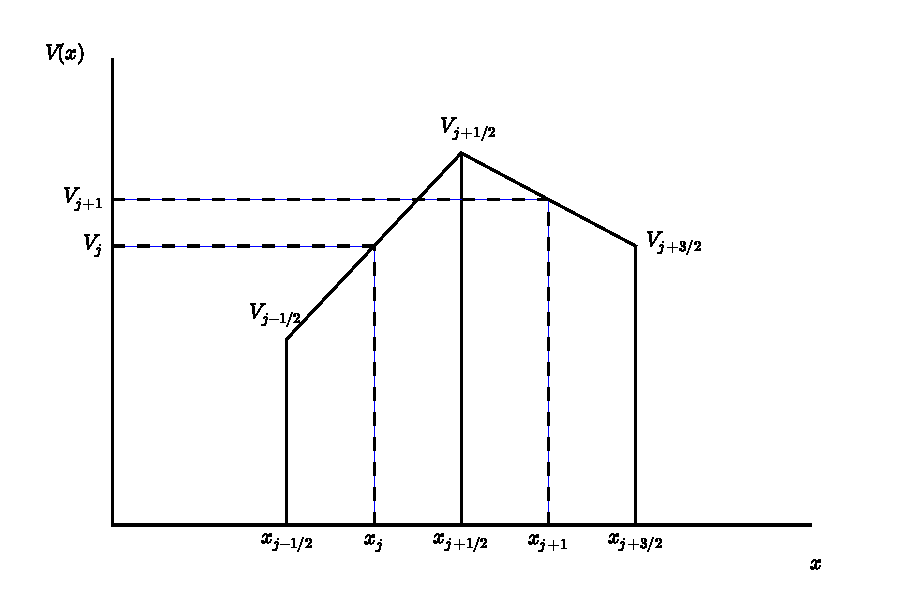
\includegraphics{figs/showcase}
    \caption{The showcase of the problem.}
\end{figure}

Take a quantum barrier in the interval $\mathcal{Q} = [x_j, x_{j+1}]$ and take the potential to be constant outside this barrier $V(x) = V_j$ in $\mathcal{C}_j = (-\infty, x_j)$ and $V(x) = V_{j+1}$ in $\mathcal{C}_{j+1} =(x_{j+1}, \infty)$. For a state $E=p^2/2m$ the time-independent Schr\"odinger equation
\begin{equation}\label{eq: main}
    -\varepsilon^2\psi''(x) + 2mV(x)\psi(x) = p^2\psi(x)
\end{equation}
has the solution
\begin{equation}\label{eq: solution}
    \psi(x) = 
    \begin{cases}
        a_1 e^{i\kappa_j(x-x_j)/\varepsilon} + b_1 e^{-i\kappa_j(x-x_j)/\varepsilon},&\quad x\in \mathcal{C}_j \\
        \psi_{\mathcal{Q}}, &\quad x\in\mathcal{Q} \\
        a_2 e^{i\kappa_{j+1}(x-x_{j+1})/\varepsilon} + b_2 e^{-i\kappa_{j+1}(x-x_{j+1})/\varepsilon},&\quad x\in \mathcal{C}_{j+1}
    \end{cases}
\end{equation}
where $\kappa_{j,j+1} = \sqrt{p^2-2mV_{j, j+1}}$ and the coefficients $a_1, b_1, a_2$ and $b_2$ are uniquely determined by the boundary conditions at $x_1$ and $x_2$. $\psi_\mathcal{Q}$ can be determined using the boundary conditions at $x_j, x_{j+1/2}$ and $x_{j+1}$ according to the paper you mention. Hence, for each momentum $p$ we may relate the solution in $\mathcal{C}_{j+1}$ with the solution $\mathcal{C}_j$ in terms of the transfer matrix $M$
\begin{equation}\label{eq: transfer matrix}
    \left(\begin{matrix}
        a_2 \\
        b_2
    \end{matrix}\right)
    = M
    \left(\begin{matrix}
        a_1 \\
        b_1
    \end{matrix}\right)
    = \left(
    \begin{matrix}
        m_{11} & m_{12} \\
        m_{21} & m_{22}
    \end{matrix}\right)
    \left(\begin{matrix}
        a_1 \\
        b_1
    \end{matrix}\right).
\end{equation}

One may also express the solutions in $\mathcal{C}_j$ and $\mathcal{C}_{j+1}$ in terms of a scattering matrix $S$ which relates the incident and scattered waves
\begin{equation}\label{eq: scattered matrix}
        \left(\begin{matrix}
        b_1 \\
        a_2
    \end{matrix}\right)
    = S
    \left(\begin{matrix}
        a_1 \\
        b_2
    \end{matrix}\right)
    = \left(
    \begin{matrix}
        r_1 & t_2 \\
        t_1 & r_2
    \end{matrix}\right)
    \left(\begin{matrix}
        a_1 \\
        b_2
    \end{matrix}\right)
    = \left(
    \begin{matrix}
        -m_{21}/m_{22} & 1/m_{22} \\
        \Delta /m_{22} & m_{12}/m{22}
    \end{matrix}\right)
    \left(\begin{matrix}
        a_1 \\
        b_2
    \end{matrix}\right)
\end{equation}
where $\Delta = \mathrm{det} M = m_{11}m_{22}-m_{12}m_{21}$. By considering the time evolution of the position density $\rho(x, t) = |\psi(x, t)|^2$ in the Schr\"odinger equation, one derives the continuity equation
\begin{equation}
    \frac{\partial}{\partial t}\rho + \nabla\cdot J = 0,
\end{equation}
where the current density $J(x)=\varepsilon m^{-1}\mathrm{Im}(\bar{\psi}\nabla\psi)$. From (\ref{eq: solution}) one has that
\begin{equation}
    J(x) = 
    \begin{cases}
        \kappa_j(|a_1|^2 - |b_1|^2)/m, \quad &x\in\mathcal{C}_j \\
        \kappa_{j+1}(|a_2|^2 - |b_2|^2)/m, \quad &x\in\mathcal{C}_{j+1}         
    \end{cases}
\end{equation}
so for a wave incident on the barrier from the left ($b_2 \equiv 0$), we have $a_2 = t_1 a_1$ and $b_1 = r_1 a_1$. It follows that the reflection coefficient $R_1$, the ratio of the reflected to incident current densities, and the transmission coefficient $T_1$, the ratio of the transmitted to incident current densities, are
\begin{equation}\label{eq: coefficients1}
    R_1 = |r_1|^2 \quad \mathrm{and}\quad T_1 = (\kappa_{j+1}/\kappa_j)|t_1|^2.
\end{equation}
Similarly, for a wave incident from the right
\begin{equation}\label{eq: coefficients2}
    R_2 = |r_2|^2 \quad \mathrm{and}\quad T_2 = (\kappa_{j}/\kappa_{j+1})|t_2|^2.
\end{equation}

For conclusion, if we have the transfer matrix $M$ as in (\ref{eq: transfer matrix}), then by using (\ref{eq: scattered matrix}) we can get $S$. Finally, using (\ref{eq: coefficients1}) or (\ref{eq: coefficients2}) we can get the transmission and reflection coefficients.

\section{Calculation of $M$}
Let us find the form of $M$. So first we will solve the equation (\ref{eq: main}) in the interval $\mathcal{Q} = [x_j, x_{j+1}]$. Notice on the half interval $[x_j, x_{j+1/2}]$, equation (\ref{eq: main}) reads:
\begin{equation}\label{eq: solveM}
    -\varepsilon^2\psi''(x) + [2m(s_j(x-x_j) + V_j)-p^2]\psi(x) = 0, \quad x\in[x_j, x_{j+1/2}].
\end{equation}

If we apply a change of variable to $x$:
\begin{equation}
    z_j(x) = \sqrt[3]{\frac{2ms_j}{\varepsilon^2}}(x - b_j),\quad x\in[x_j, x_{j+1/2}]
\end{equation}
where $b_j = x_j + p^2/2ms_j - V_j/s_j$. Then the equation (\ref{eq: solveM})) changes to
\begin{equation}
    \psi''(z_j) - z_j\psi(z_j) = 0
\end{equation}
which is the standard Airy equation. The solution of this equation is the airy function:
\begin{equation}
    \psi_\mathcal{Q}(z_j(x)) = C_j^{(1)}\mathrm{Ai}(z_j(x)) + C_j^{(2)}\mathrm{Bi}(z_j(x)).
\end{equation}

To determine the coefficients, notice the continuity of $\psi$ and its derivative $\psi'$ at $x_j$:
\begin{equation}\label{eq: M(x)}
    \left(
    \begin{matrix}
        1 & 1 \\
        i\kappa_j/\varepsilon & -i\kappa_j/\varepsilon
    \end{matrix}\right)
    \left(\begin{matrix}
        a_1 \\
        b_1
    \end{matrix}\right)
    =
    \left(\begin{matrix}
        \mathrm{Ai}(z_j(x_j)) & \mathrm{Bi}(z_j(x_j)) \\
        \sqrt[3]{\frac{2ms_j}{\varepsilon^2}}\mathrm{Ai}'(z_j(x_j)) & \sqrt[3]{\frac{2ms_j}{\varepsilon^2}}\mathrm{Bi}'(z_j(x_j))
    \end{matrix}\right)
    \left(
    \begin{matrix}
        C_j^{(1)} \\
        C_j^{(2)}
    \end{matrix}\right).
\end{equation}
For convenience, we wil denote:
\begin{equation}
    M_j(x) \equiv \left(\begin{matrix}
        \mathrm{Ai}(z_j(x)) & \mathrm{Bi}(z_j(x)) \\
        \sqrt[3]{\frac{2ms_j}{\varepsilon^2}}\mathrm{Ai}'(z_j(x)) & \sqrt[3]{\frac{2ms_j}{\varepsilon^2}}\mathrm{Bi}'(z_j(x))
    \end{matrix}\right)
\end{equation}
and 
\begin{equation}
    P_j \equiv  \left(
    \begin{matrix}
        1 & 1 \\
        i\kappa_j/\varepsilon & -i\kappa_j/\varepsilon
    \end{matrix}\right).
\end{equation}
Then equation (\ref{eq: M(x)}) can be rewritten as 
\begin{equation}
        \left(\begin{matrix}
        a_1 \\
        b_1
    \end{matrix}\right)
    = P_jM_j(x_j)
    \left(\begin{matrix}
        C_j^{(1)} \\
        C_j^{(2)}
    \end{matrix}\right).
\end{equation}

In the same way, we have at point $x_{j+1/2}$
\begin{equation}
    M_j(x_{j+1/2}=x_j+\Delta x/2)   \left(\begin{matrix}
        C_j^{(1)} \\
        C_j^{(2)}
    \end{matrix}\right)
    =
    M_{j+1}(x_{j+1/2}=x_j+\Delta x/2)
    \left(\begin{matrix}
        C_{j+1}^{(1)} \\
        C_{j+1}^{(2)}
    \end{matrix}\right) 
\end{equation}
and also at point $x_{j+1}$
\begin{equation}
        M_{j+1}(x_{j+1})
    \left(\begin{matrix}
        C_{j+1}^{(1)} \\
        C_{j+1}^{(2)}
    \end{matrix}\right) 
    = P_{j+1}
    \left(\begin{matrix}
        a_2 \\
        b_2
    \end{matrix}\right).
\end{equation}
Combine all the equations above (17), (18) and (19) we have
\begin{equation}
        \left(\begin{matrix}
        a_1 \\
        b_1
    \end{matrix}\right)
    =
    P_j^{-1}M_j(x_j)M_j^{-1}(x_{j+1/2})M_{j+1}(x_{j+1/2})M_{j+1}^{-1}(x_{j+1})P_{j+1}
        \left(\begin{matrix}
        a_2 \\
        b_2
    \end{matrix}\right).
\end{equation}
Notice the difference between $M_j(x_j)$ and $M^{-1}_j(x_{j+1/2})$, also the difference between $M_{j+1}(x_{j+1/2})$ and $M^{-1}_{j+1}(x_{j+1})$, thus these matrices can't be cancelled.

Finally, our $M$ is 
\begin{equation}
    M = P_j^{-1}M_j(x_j)M_j^{-1}(x_{j+1/2})M_{j+1}(x_{j+1/2})M_{j+1}^{-1}(x_{j+1})P_{j+1}
\end{equation}

\section{Conclusion}

To calculate the transmission and reflection coefficients at $x_{j+1/2}$. First, we calculate $M$ using (21) in which $M_{j}$ and $P_j$ are defined by (15) and (16). Then we calculate $S$ using (5) to get $r_1$, $t1$, $r_2$ and $t_2$. Finally, apply (8) or (9) to get the result.


















\end{document}